%\{ {\it  sp1d\_ch3\_1.tex} \}

\subsubsection {H/P Convergence Test for Two-dimensional Solution}

In this section we present the convergence behavior in both $h$
refinement and $p$ refinement for the following steady-state
Poisson differential equation:
\begin{equation}
\label{pois_sin}
-r^2 \frac{\partial}{\partial r} (\sigma \frac{\partial}{\partial r}u) - r \sigma \frac{\partial}{\partial r}u - \sigma \frac{\partial^2}{\partial \theta^2}u = r \cos \theta \left[ -4 r \pi \cos S_r + \{4\pi^2 + 1\} \sin S_r \right],
\end{equation}
for all $r \in [1, 2], \theta \in [0, 2\pi]$ with $\sigma(r) = r$.

The analytic solution is known to be
\begin{equation}
u(r, \theta) = \sin S_r \cos \theta,
\end{equation}
where $S_r = 2\pi (r-1) - \pi$.

The numerical that has same shape as exact solutions are shown in
figure (\ref{sinsol}) with 2 different viewpoint.

\begin{figure}[h]
    \begin{center}
    \epsfig{file = Doc-Report_Fwd2D/figs_dn/sinDN_e10_t8.eps, width = 5cm} %Error: 4.7740e-15
    \epsfig{file = Doc-Report_Fwd2D/figs_dn/sinDN_e10_t8_1.eps, width = 5cm}
    \caption{\label{sinsol}Numerical solution of equation (\ref{pois_sin}) with polynomial order $P=10$, $10$ equidistance elements. The difference to exact solution is 4.7740e-15 in terms of $L_{\infty}$ norm.}
    \end{center}
\end{figure}

\begin{figure}[h]
    \begin{center}
    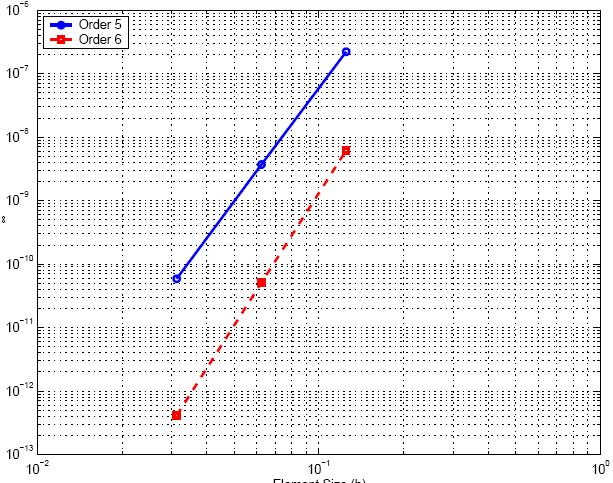
\epsfig{file = Doc-Report_Fwd2D/figs_dn/sinDNhconv.eps, width = 8.3cm}
    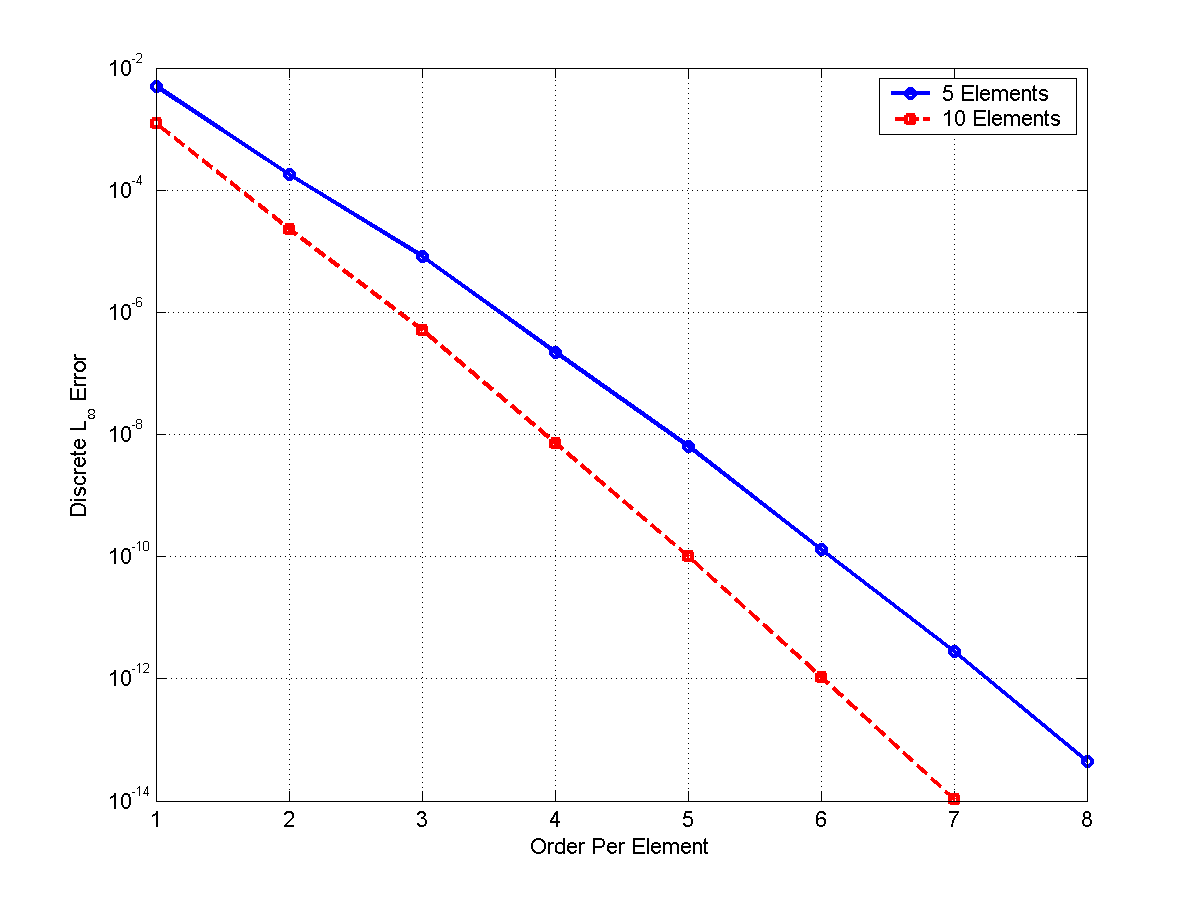
\epsfig{file = Doc-Report_Fwd2D/figs_dn/sinDNpconv.eps, width = 8.3cm}
    \caption{\label{sinDNconv}
(Left) Convergence with respect to discrete $L^{\infty}$ norm as a
function of size of elements. This test is performed using the
h-type extension with fixed polynomial order 5 and 6 respectively.
Error on the Log-Log axis is demonstrating the algebraic
convergence of the h-type extension. (Right) Convergence w.r.t.
$L^{\infty}$ norm as a function of size of polynomial order in
semi-Log plot. It shows the exponential convergence of p-type
extension for smooth solution. Two tests are performed for p-type
extension with element length $0.2$ and $0.1$. }
\end{center}
\end{figure}


\begin{table}[h]
\centering \caption{\label{hconv2t} This table shows the
convergence of h-type (left) and p-type (right) resolution control
done above Figure (\ref{sinDNconv}). We can see the slope of each
case is $P+1$ of order $P$. }
\begin{tabular}{|c|c|c|} \hline
    Polynomial order&Error($L^{\infty}$)&Slope   \\ \hline \hline
    5&$9.3603e-013$ &$5.9406$ \\ \hline
    6&$8.6542e-014$ &$6.9402$ \\ \hline
\end{tabular}
\hspace{.5in}
\begin{tabular}{|c|c|} \hline
    Element Size&Error($L^{\infty}$)\\ \hline
    0.2&$1.9385e-012$  \\ \hline
    0.1&$3.4611e-013$  \\ \hline
\end{tabular}

\end{table}
